%%\documentclass[a4paper,12pt,oneside]{llncs}
\documentclass[12pt,letterpaper]{article}
\usepackage[right=2cm,left=3cm,top=2cm,bottom=2cm,headsep=0cm]{geometry}

%%%%%%%%%%%%%%%%%%%%%%%%%%%%%%%%%%%%%%%%%%%%%%%%%%%%%%%%%%%
%% Juego de caracteres usado en el archivo fuente: UTF-8
\usepackage{ucs}
\usepackage[utf8x]{inputenc}

%%%%%%%%%%%%%%%%%%%%%%%%%%%%%%%%%%%%%%%%%%%%%%%%%%%%%%%%%%%
%% Juego de caracteres usado en la salida dvi
%% Otra posibilidad: \usepackage{t1enc}
\usepackage[T1]{fontenc}

%%%%%%%%%%%%%%%%%%%%%%%%%%%%%%%%%%%%%%%%%%%%%%%%%%%%%%%%%%%
%% Ajusta maergenes para a4
%\usepackage{a4wide}

%%%%%%%%%%%%%%%%%%%%%%%%%%%%%%%%%%%%%%%%%%%%%%%%%%%%%%%%%%%
%% Uso fuente postscript times, para que los ps y pdf queden y pequeños...
\usepackage{times}

%%%%%%%%%%%%%%%%%%%%%%%%%%%%%%%%%%%%%%%%%%%%%%%%%%%%%%%%%%%
%% Posibilidad de hipertexto (especialmente en pdf)
%\usepackage{hyperref}
\usepackage[bookmarks = true, colorlinks=true, linkcolor = black, citecolor = black, menucolor = black, urlcolor = black]{hyperref}

%%%%%%%%%%%%%%%%%%%%%%%%%%%%%%%%%%%%%%%%%%%%%%%%%%%%%%%%%%%
%% Graficos 
\usepackage{graphics,graphicx}

%%%%%%%%%%%%%%%%%%%%%%%%%%%%%%%%%%%%%%%%%%%%%%%%%%%%%%%%%%%
%% Ciertos caracteres "raros"...
\usepackage{latexsym}

%%%%%%%%%%%%%%%%%%%%%%%%%%%%%%%%%%%%%%%%%%%%%%%%%%%%%%%%%%%
%% Matematicas aun más fuertes (american math dociety)
\usepackage{amsmath}

%%%%%%%%%%%%%%%%%%%%%%%%%%%%%%%%%%%%%%%%%%%%%%%%%%%%%%%%%%%
\usepackage{multirow} % para las tablas
\usepackage[spanish,es-tabla]{babel}

%%%%%%%%%%%%%%%%%%%%%%%%%%%%%%%%%%%%%%%%%%%%%%%%%%%%%%%%%%%
%% Fuentes matematicas lo mas compatibles posibles con postscript (times)
%% (Esto no funciona para todos los simbolos pero reduce mucho el tamaño del
%% pdf si hay muchas matamaticas....
\usepackage{mathptm}

%%% VARIOS:
%\usepackage{slashbox}
\usepackage{verbatim}
\usepackage{array}
\usepackage{listings}
\usepackage{multirow}

%% MARCA DE AGUA
%% Este package de "draft copy" NO funciona con pdflatex
%%\usepackage{draftcopy}
%% Este package de "draft copy" SI funciona con pdflatex
%%%\usepackage{pdfdraftcopy}
%%%%%%%%%%%%%%%%%%%%%%%%%%%%%%%%%%%%%%%%%%%%%%%%%%%%%%%%%%%
%% Indenteacion en español...
\usepackage[spanish]{babel}

\usepackage{listingsutf8}
% Para escribir código en C
% \begin{lstlisting}[language=C]
% #include <stdio.h>
% int main(int argc, char* argv[]) {
% puts("Hola mundo!");
% }
% \end{lstlisting}


\title{Práctica 3}
\author{Jesús Rodríguez Heras\\
	Arantzazu Otal Alberro}

\begin{document}
	
	\maketitle
%	\begin{abstract} %Poner esto en todas las prácticas de PCTR
%%		\begin{center}
%%			\noindent
%			
%%		\end{center}
%	\end{abstract}
	\thispagestyle{empty}
	\newpage
	
%	\tableofcontents
%	\newpage
	
	%%\listoftables
	%%\newpage
	
	%%\listoffigures
	%%\newpage
	
	%%%% REAL WORK BEGINS HERE:
	
	%%Configuracion del paquete listings
	\lstset{language=bash, numbers=left, numberstyle=\tiny, numbersep=10pt, firstnumber=1, stepnumber=1, basicstyle=\small\ttfamily, tabsize=1, extendedchars=true, inputencoding=utf8/latin1, breaklines=true}
	
\section{Instalación de máquinas virtuales mediante Vagrant}
En esta primera parte vamos a crear el entorno de trabajo, consiste en dos redes internas, conectadas al exterior mediante un router.
\begin{itemize}
	\item La primera red tendrá el rango de IPs 192.168.2.0.
	\item La segunda red tendrá el rango de IPs 192.168.3.0.
\end{itemize}

Cada red tendrá un par de máquinas virtuales (no hace falta conectarlas todas de forma simultánea). Además, las redes solo tendrán acceso al exterior a través de la máquina que actúa como router.

En este ejercicio se deberá:
\begin{itemize}
	\item \textbf{Crear el entorno de red mediante un único fichero Vagrant.}
	\lstinputlisting[language=Ruby]{../Vagrantfile}
	
	\item \textbf{Configurar el cortafuegos para que de acceso al exterior.} \\
	Para configurar el cortafuegos, primero debemos deshabilitar la interfaz de red que nos permite salir a Internet desde cada una de las máquinas de las redes. Para ello, identificamos la interfaz que queremos deshabilitar (en nuestro caso, \texttt{eth0}).
	
	Si deshabilitamos esta interfaz directamente, tendremos el problema de que la terminal se quedará colgada porque estamos conectados por SSH a esa interfaz, entonces debemos habilitar la conexión SSH desde la otra interfaz. Para ello nos dirigimos al fichero \texttt{sshd\_config} con:
	\begin{center}
		\texttt{sudo nano /etc/ssh/sshd\_config}
	\end{center}
	
	Descomentamos la línea que dice \texttt{PasswordAuthentication yes}. Luego, reiniciamos el servicio SSH con el siguiente comando:
	\begin{center}
		sudo /etc/init.d/ssh restart
	\end{center}

	Después de esto, ya podemos conectarnos desde la máquina que actúa como router/cortafuegos.
	
	Es hora de entrar en la máquina cortafuegos y conectarnos por SSH a cada una de las máquinas. Una vez dentro de las máquinas servidoras usamos el siguiente comando para deshabilitar la interfaz de red externa:
	\begin{center}
		\texttt{sudo ifconfig eth0 down}
	\end{center}
	
	También debemos activar el ip forward en el router para tener conectividad entre las máquinas de las diferentes redes. Para ello usamos el comando:
	\begin{center}
		\texttt{sudo echo 1 > /proc/sys/net/ipv4/ip\_forward}
	\end{center}
	
	A continuación, establecemos la puerta de enlace como la interfaz que tenemos en la máquina que hace de router. Para ello usamos el comando:
	\begin{center}
		\texttt{sudo route add default gw 192.168.x.1 eth1}
	\end{center}

	Siendo \texttt{x} la red a la que pertenece cada máquina, y \texttt{eth1} la interfaz de la red interna.
	\begin{figure}[h]
		\centering
		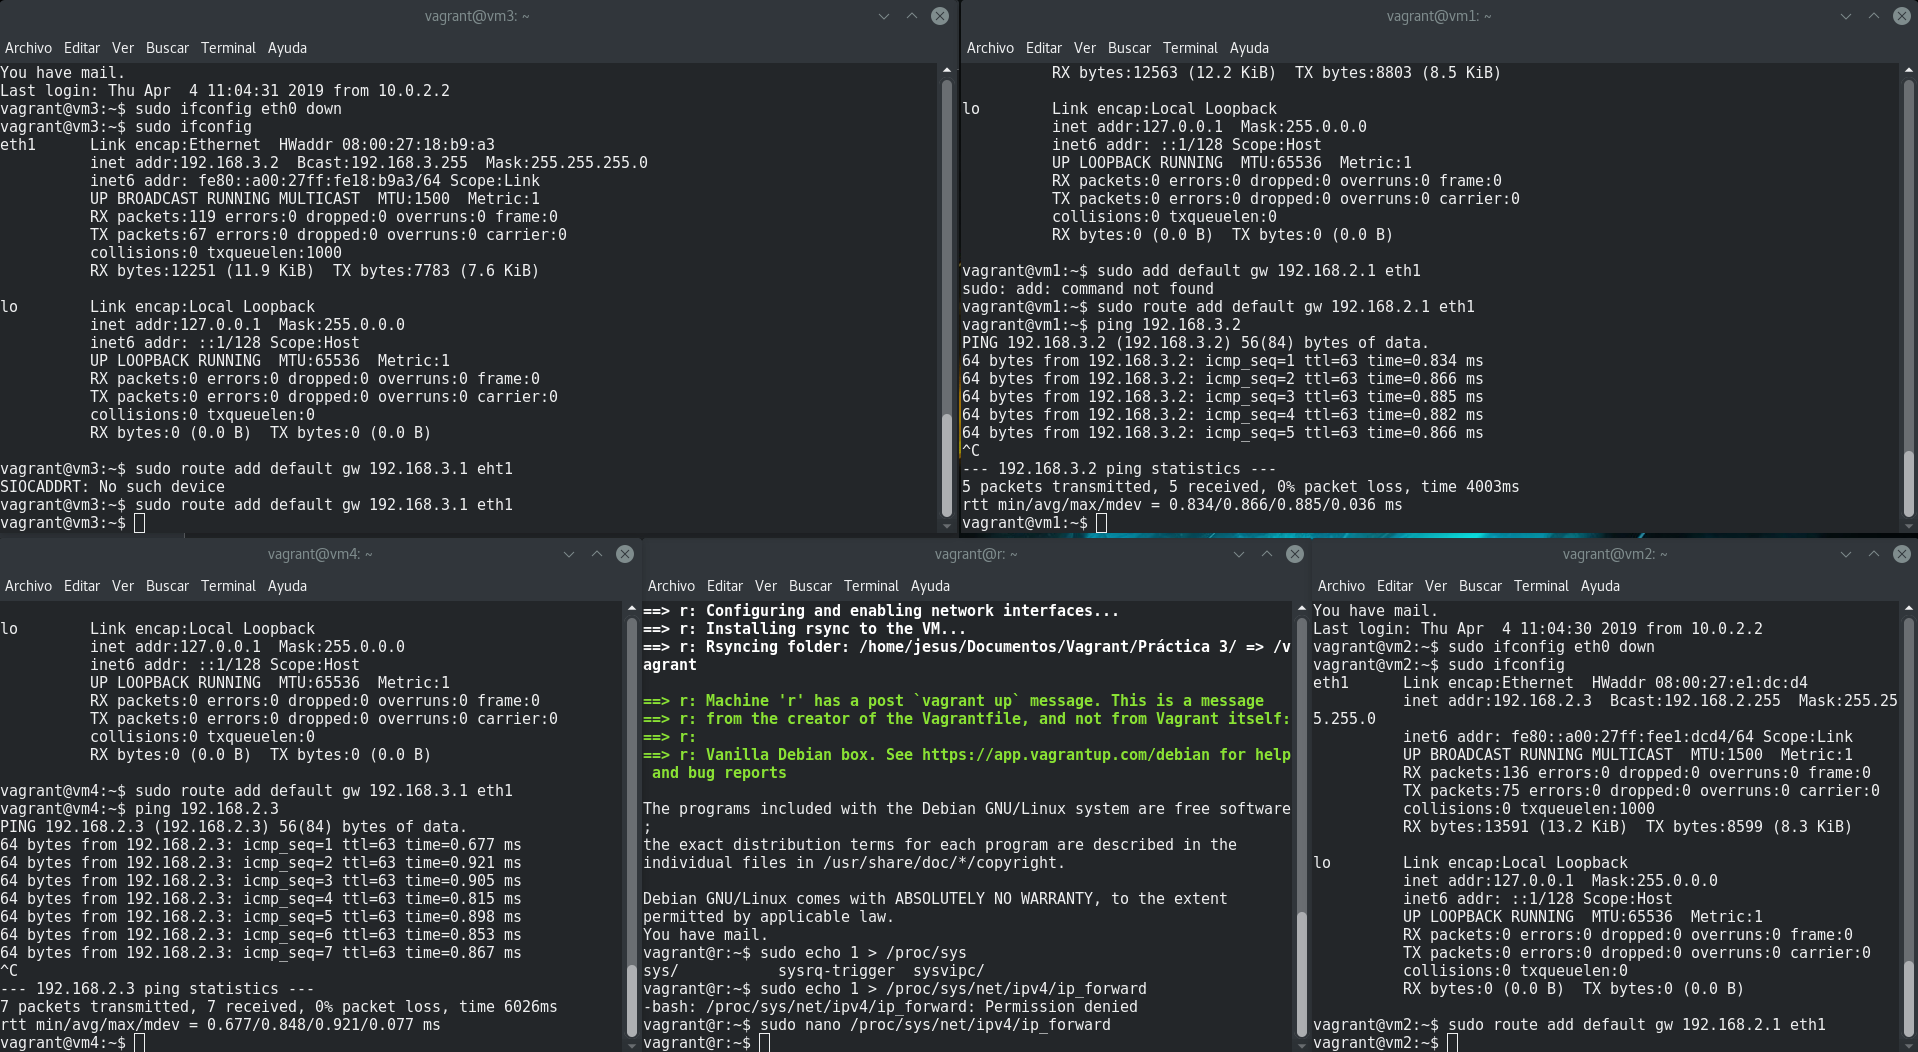
\includegraphics[scale=0.25]{Ping.png}
		\caption{En esta imagen se ve como la vm4 (red 2) hace ping a la vm2 (red 1) y la vm1 (red1) hace ping a la vm3 (red 2).}
	\end{figure}
	
	Lo siguiente es habilitar el enrutamiento a partir de la máquina router al resto de máquinas. El estado inicial es el siguiente:
	\newpage
	\begin{figure}[h]
		\centering
		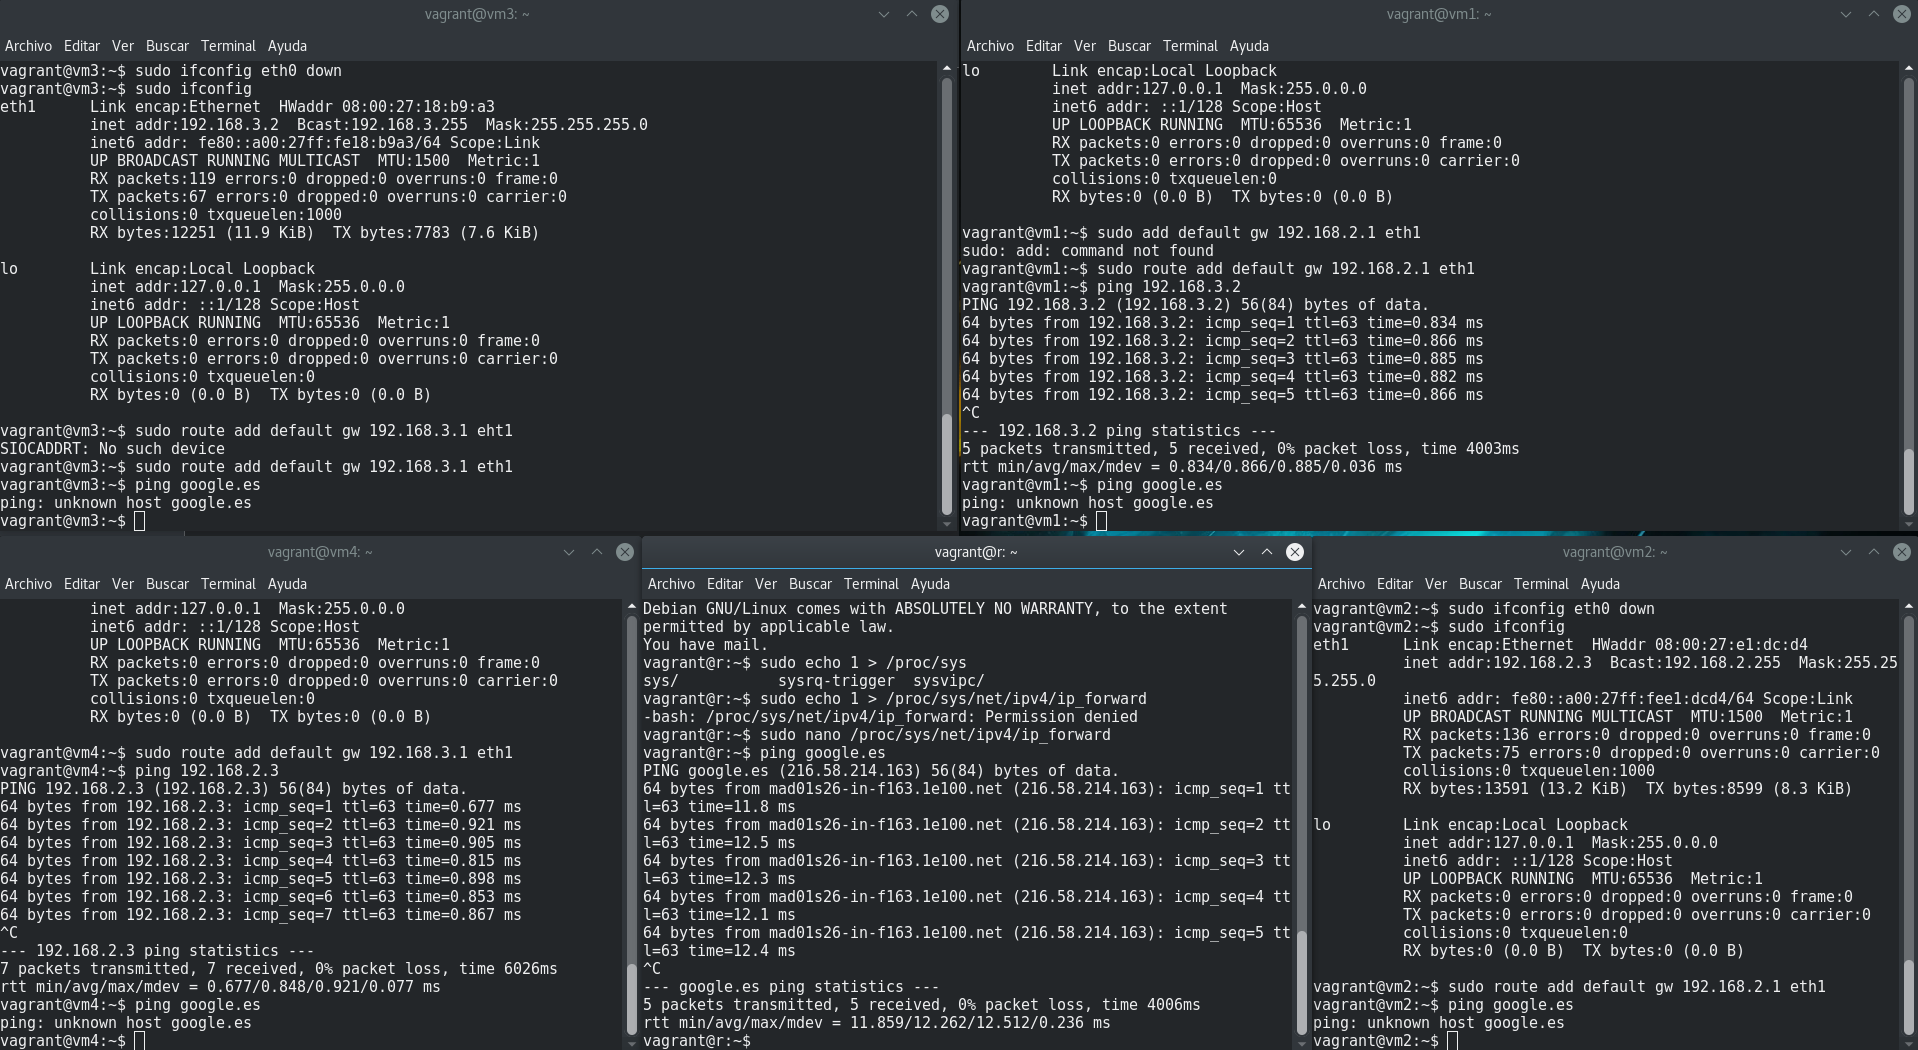
\includegraphics[scale=0.25]{Ping2.png}
		\caption{En esta imagen se ve como todas las máquinas intentan hacer ping a \texttt{google.es} pero la única que lo consigue es la máquina r (router/cortafuegos).}
	\end{figure}
	\textcolor{white}{.}
	\newpage
	 Para habilitar el enrutamiento usamos el comando en la máquina router/cortafuegos:
	 \begin{center}
	 	\texttt{sudo iptables -t nat -A \\POSTROUTING -o eth0 -j MASQUERADE}
	 \end{center}
 	 
	 Una vez hecho eso, el resultado es el siguiente:
	 \begin{figure}[h]
	 	\centering
	 	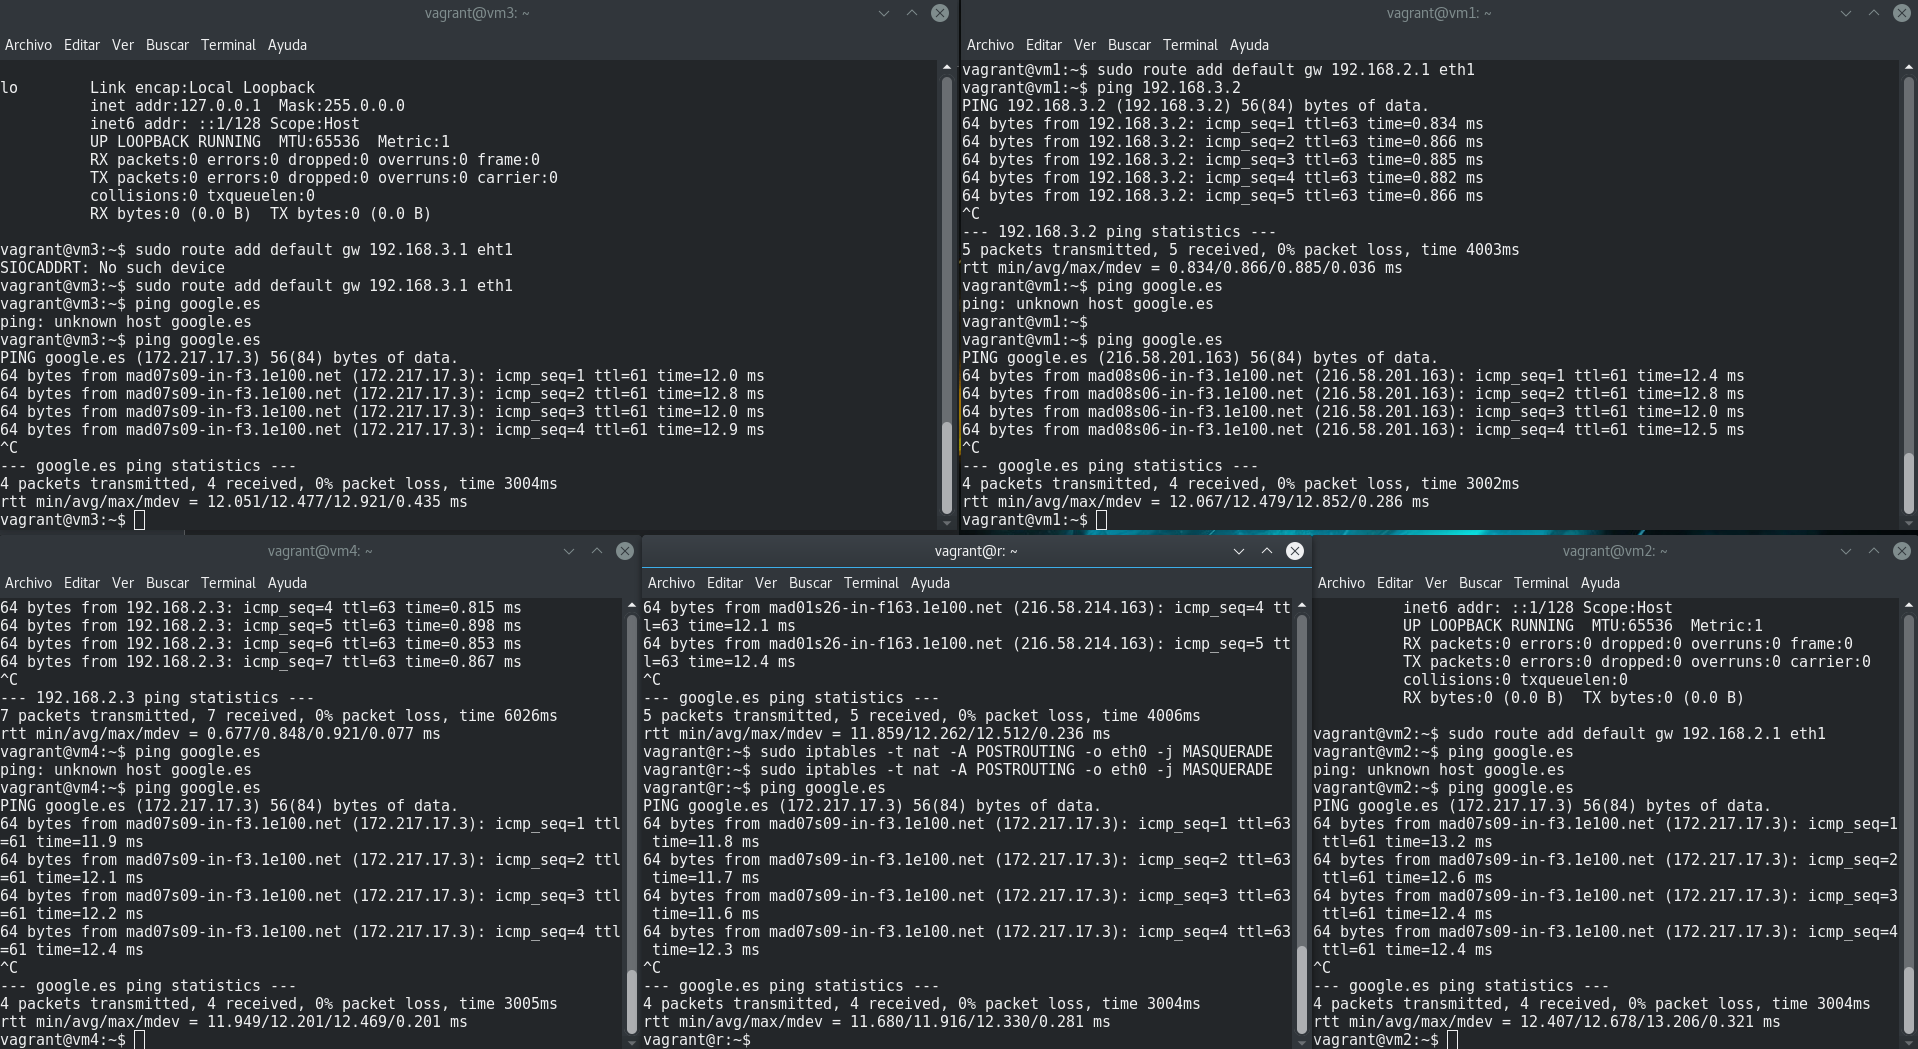
\includegraphics[scale=0.25]{Ping3.png}
	 	\caption{Una vez habilitado el enrutamiento, todas las máquinas tienen acceso a Internet.}
	 \end{figure}
	
	\newpage
	\item \textbf{Configurar manualmente los clientes de las redes para que se puedan conectar al servidor.} \\
	Solo con poner la puerta de enlace y el ip forwarding estaría hecho y ya se ha hecho en el apartado anterior.
\end{itemize}

\newpage
\section{Servidor DHCP}
Instalar un servidor DHCP en el cortafuegos. Además, se deberá modificar el fichero Vagrant, para que en lugar de establecer una IP privada, la IP se asigne mediante DHCP.

También se puede probar dejando la IP privada y comprobando el funcionamiento del servidor DHCP mediante el cliente DHCP.

El servidor DHCP deberá asignar direcciones IP a cada una de las redes internas. Además, una máquina de la segunda red tendrá que tener una dirección fija.

Tras la configuración, mostrar el estado de los prestamos realizados por el servidor DHCP.

Para instalar el servidor DHCP introducimos el siguiente comando:
\begin{center}
	\texttt{sudo apt-get install isc-dhcp-server}
\end{center}


Configuramos las subredes en el archivo \texttt{/etc/dhcp/dhcpd.conf} abriendolo con el comando:
\begin{center}
	\texttt{sudo nano /etc/dhcp/dhcpd.conf}
\end{center}
\begin{figure}[h]
	\centering
	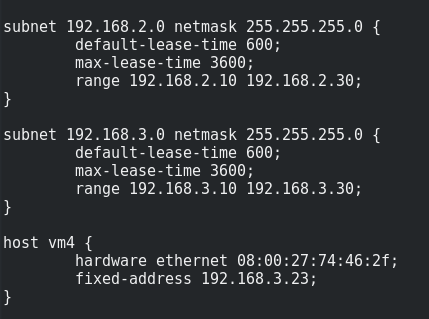
\includegraphics[scale=0.8]{DHCP2.png}
	\caption{Configuración de las subredes del DNS}
\end{figure}

Ahora, reiniciamos el servidor dhcp con:
\begin{center}
	\texttt{sudo /etc/init.d/isc-dhcp-server restart}
\end{center}

Para comprobar el estado del servidor dhcp usaremos el siguiente comando:
\begin{center}
	\texttt{sudo /etc/init.d/isc-dhcp-server status}
\end{center}

A continuación, pedimos una IP al servidor DHCP desde las otras máquinas con:
\begin{center}
	\texttt{sudo dhclient -v}
\end{center}
\newpage
\begin{figure}[h]
	\centering
	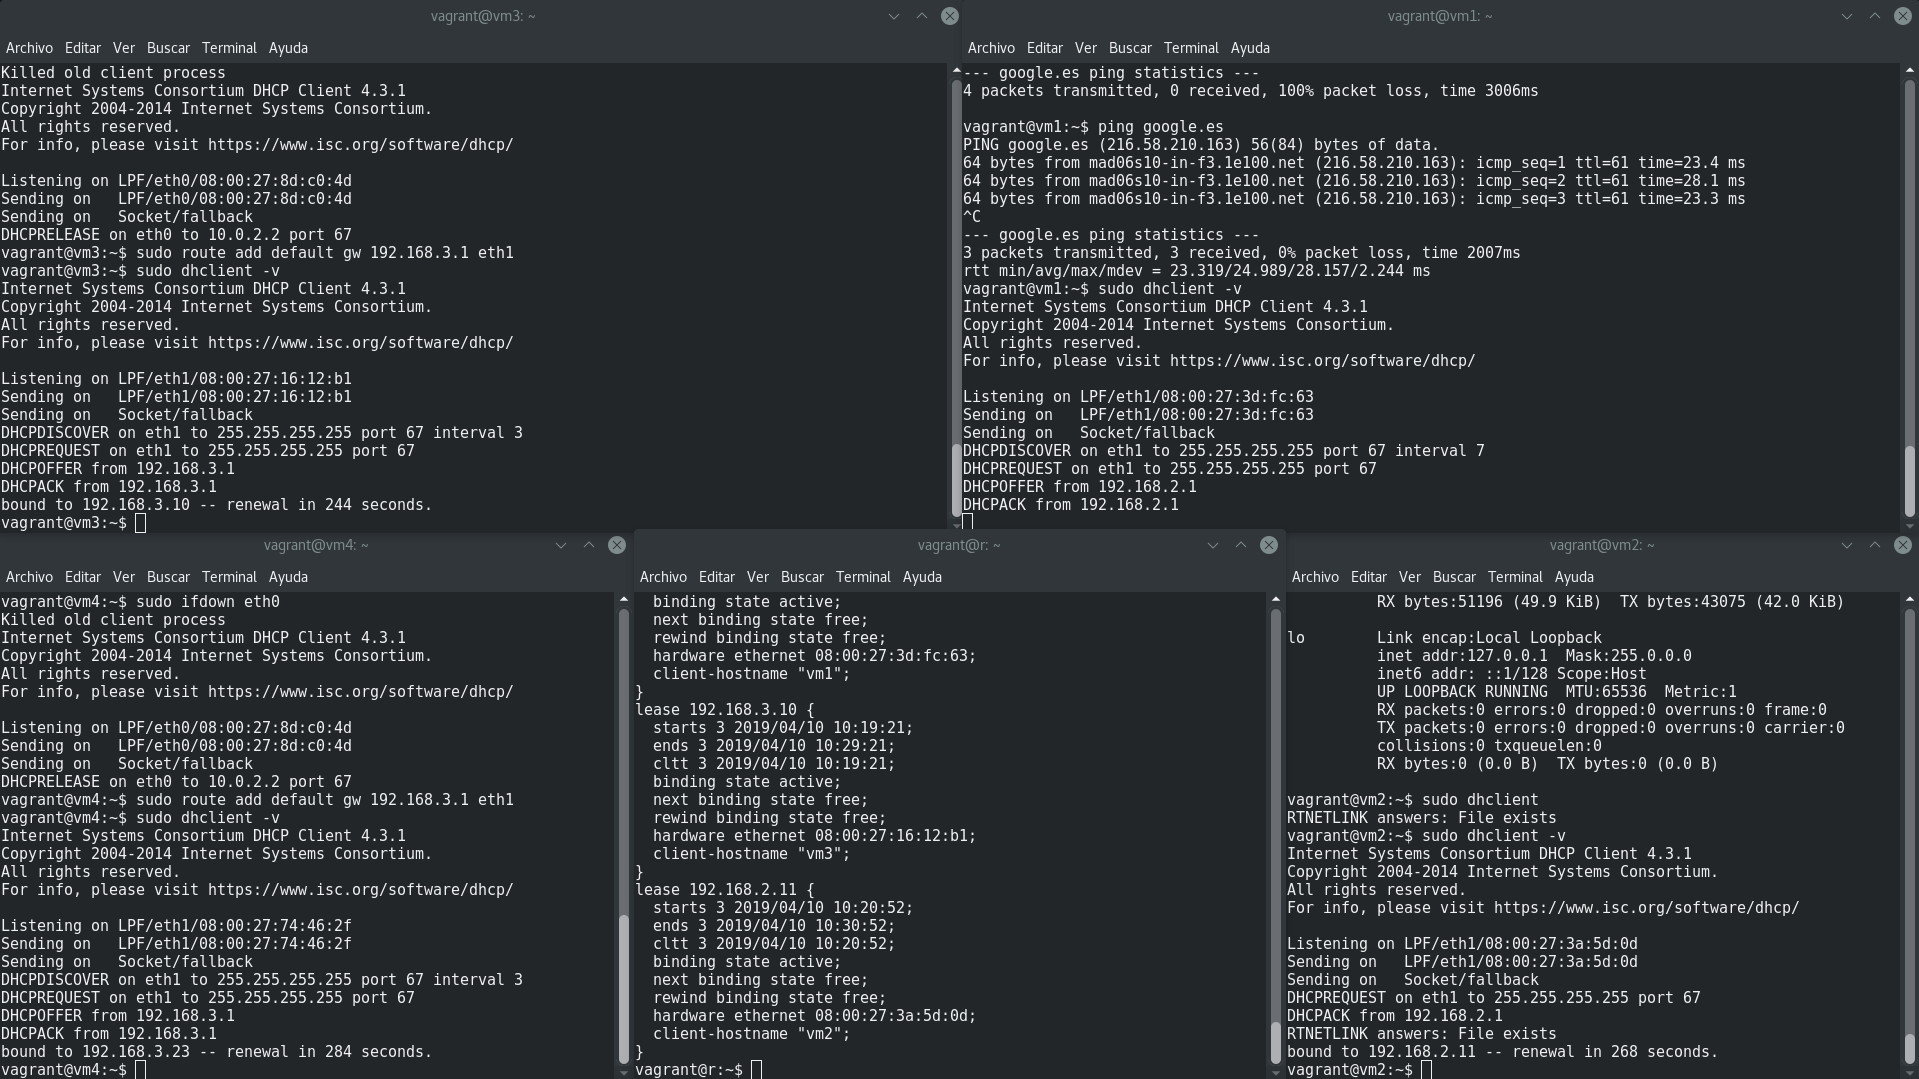
\includegraphics[scale=0.25]{DHCP1.png}
	\caption{Petición de IP desde las máquinas al servidor DHCP}
\end{figure}

Para ver las direcciones IP cedidas por el servidor DHCP usamos:
\begin{center}
	\texttt{sudo cat /var/lib/dhcp/dhcpd.leases}
\end{center}
\newpage
\begin{figure}[h]
	\centering
	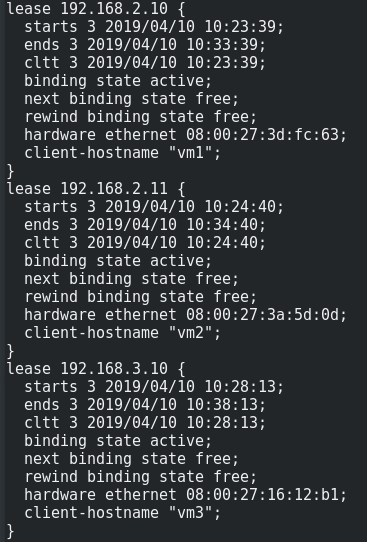
\includegraphics[scale=0.8]{DHCP3.png}
	\caption{Vista de las direcciones IP cedidas por el servidor DHCP}
\end{figure}

\section{Servidor DNS}
Configurar la máquina central (router) para que actúe como DNS. Para ello, volveremos a configurar las máquinas con IP fijas, bien por DHCP o bien a mano.
\begin{itemize}
	\item La máquina 1 de la red 1 tendrá por nombre \texttt{vm1.net1.uca.es}.
	\item La máquina 2 de la red 1 tendrá por nombre \texttt{vm2.net1.uca.es}.
	\item La máquina 1 de la red 2 tendrá por nombre \texttt{www.as.uca.es}, además, tendrá que responder bajo el nombre de \texttt{ftp.as.uca.es}.
	\item La máquina 2 de la red 2 tendrá por nombre \texttt{bd.as.uca.es}.
\end{itemize}

Ahora cambiamos el servidor de zona y el fichero de zona:
\begin{center}
	\texttt{/etc/bind/named.conf.default-zones}
\end{center}
\begin{figure}[h]
	\centering
	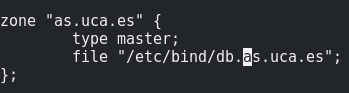
\includegraphics[scale=0.75]{Zona.png}
	\caption{Fichero de zona}
\end{figure}
%\newpage
\begin{figure}[h]
	\centering
	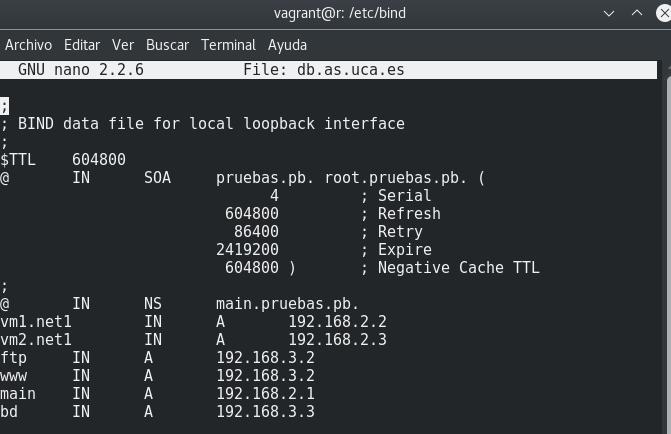
\includegraphics[scale=0.65]{BD.png}
	\caption{Archivo \texttt{db.as.uca.es}}
\end{figure}

Por último, cambiamos el servidor DNS del resto de máquinas en el fichero \texttt{/etc/resolv.conf} con el siguiente comando:
\begin{center}
	\texttt{sudo nano /etc/resolv.conf}
\end{center}

Y cambiamos el servidor DNS por \texttt{192.168.2.1}.
\newpage
\begin{figure}[h]
	\centering
	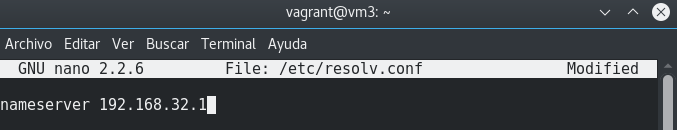
\includegraphics[scale=0.5]{Nameserver.png}
	\caption{Archivo \texttt{/etc/resolv.conf} de las máquinas servidoras}
\end{figure}

Una vez realizados los cambios necesarios en el archivo de zona y en el archivo DNS, probamos a hacer ping a los nombres de dominio, para que el servidor DNS sea el que resuelva la dirección:
\begin{figure}[h]
	\centering
	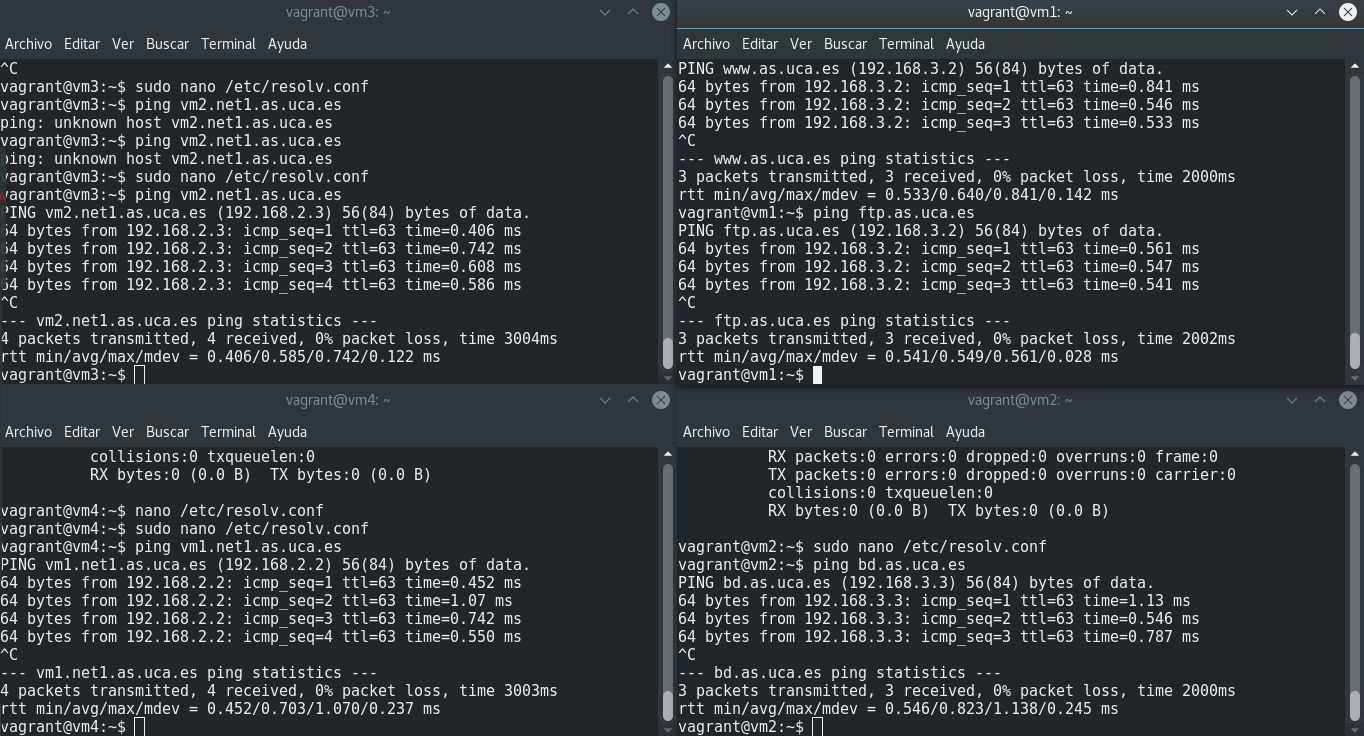
\includegraphics[scale=0.345]{Final.png}
	\caption{Máquinas servidoras haciendo ping a los dominios}
\end{figure}


\end{document}